
\subsection{Otras Métricas }

\begin{frame}
  \frametitle{Otras métricas}
  \framesubtitle{de mimetización acústico-prosódica}

  \begin{figure}
    \includegraphics[scale=0.40]{images/types_of_entrainment.jpg}
  \end{figure}

  \begin{itemize}
    \item Algunas métricas captan sólo la convergencia de los factores
    \item Otras capturan la sincronía: la variación turno a turno.
    \item Algunas métricas requieren de anotaciones manuales sobre las conversaciones, por ejemplo patrones de entonación.
  \end{itemize}

\end{frame}


\begin{frame}
  \frametitle{Problema del alineamiento de tiempo}

  \begin{figure}[t]
    
\includegraphics[scale=0.40]{images/conversation_turns.pdf}
  \end{figure}
  Uno de los problemas que tenemos a la hora de construir métricas de mimetización

  \begin{itemize}
    \item ¿Cómo comparamos los diferentes turnos de una conversación?
    \item Comparar uno a uno es un enfoque simplista y no representativo de la realidad
  \end{itemize}
\end{frame}


\subsection{Método TAMA}

\begin{frame}
  \frametitle{Método TAMA}
  \framesubtitle{Time Aligned Moving Average}
  \begin{itemize}
    \item Introducido en Kousidis et al (2008) \footnote{Spyros Kousidis, David Dorran, Ciaran McDonnell, and Eugene Coyle. Times series analysis of acoustic feature convergence in human dialogues. In
Proceedings of Interspeech, 2008.}
    \item Construímos en primer lugar series de tiempo para cada uno de los hablantes, dada una variable acústico/prosódica.
    \item Mimetización se define como una función de estas dos series.
  \end{itemize}
\end{frame}


\begin{frame}
  \frametitle{Series de Tiempo}
  \framesubtitle{¿Qué es una serie de tiempo?}

  \begin{figure}[t]
    \includegraphics[scale=0.35]{images/oil_price.jpg}
  \end{figure}

  \begin{itemize}
     \item En términos coloquiales, una serie de tiempo es una colección de datos temporales.
     \item El tipo de análisis que vamos a efectuar es propio de Economía y Ciencias de la Atmósfera.
     \item ¡Mucho más manejables que una sucesión de turnos!
   \end{itemize}
\end{frame}



\begin{frame}
  \frametitle{Método TAMA}
  \framesubtitle{Cómo construyo la serie de tiempo (dada una variable a-p)}

  \begin{columns}
    \column{0.50\textwidth}
    \begin{figure}[t]
      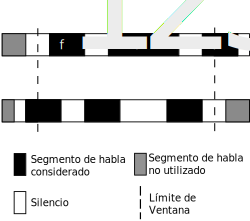
\includegraphics[width=\textwidth]{images/tama_improved.pdf}
    \end{figure}

    \column{0.50\textwidth}
    \begin{enumerate}
      \item Partimos la conversación en ventanas solapadas.
      \item Para cada ventana: calculamos un promedio ponderado del valor de la variable acústico-prosódica en cada segmento de habla
    \end{enumerate}

    \begin{align*}
      \mu = \sum\limits_{i=1}^N f_i \frac{d_i}{D} \text{ con } D = \sum\limits_{i=1}^N d_i
    \end{align*}
  \end{columns}

\end{frame}


\begin{frame}
  \frametitle{Método TAMA}
  \framesubtitle{¿Y el mimetización?}
  \begin{columns}
  \column{0.33\textwidth}
  \begin{figure}[t]
    \includegraphics[scale=0.28]{images/time_plot.png}
  \end{figure}
  \begin{figure}[t]
    \includegraphics[scale=0.28]{images/cross_correlogram.png}
  \end{figure}
  \column{0.66\textwidth}
  \begin{enumerate}
    \item Ya tenemos la serie de tiempo
    \item ¿Cómo calculamos la mimetización?
    \item Función de correlación cruzada: mide la influencia de una serie sobre otra.
    \item Similar a la correlación, pero aplicando un desplazamiento en alguna de las dos series.
    \item Los valores significativos de esta son los que se consideran los valores de \emph{mimetización} (si es que los hay)
    \item Si el valor es positivo, lo consideramos mimetización.
    \item Si el valor es negativo, lo consideramos antimimetización.
  \end{enumerate}

  \end{columns}
\end{frame}
